\documentclass[border=8pt]{standalone}
\usepackage{tikz}
\usepackage{amsmath,amssymb}
\usetikzlibrary{arrows.meta,calc,positioning}
\pagestyle{empty}

\begin{document}
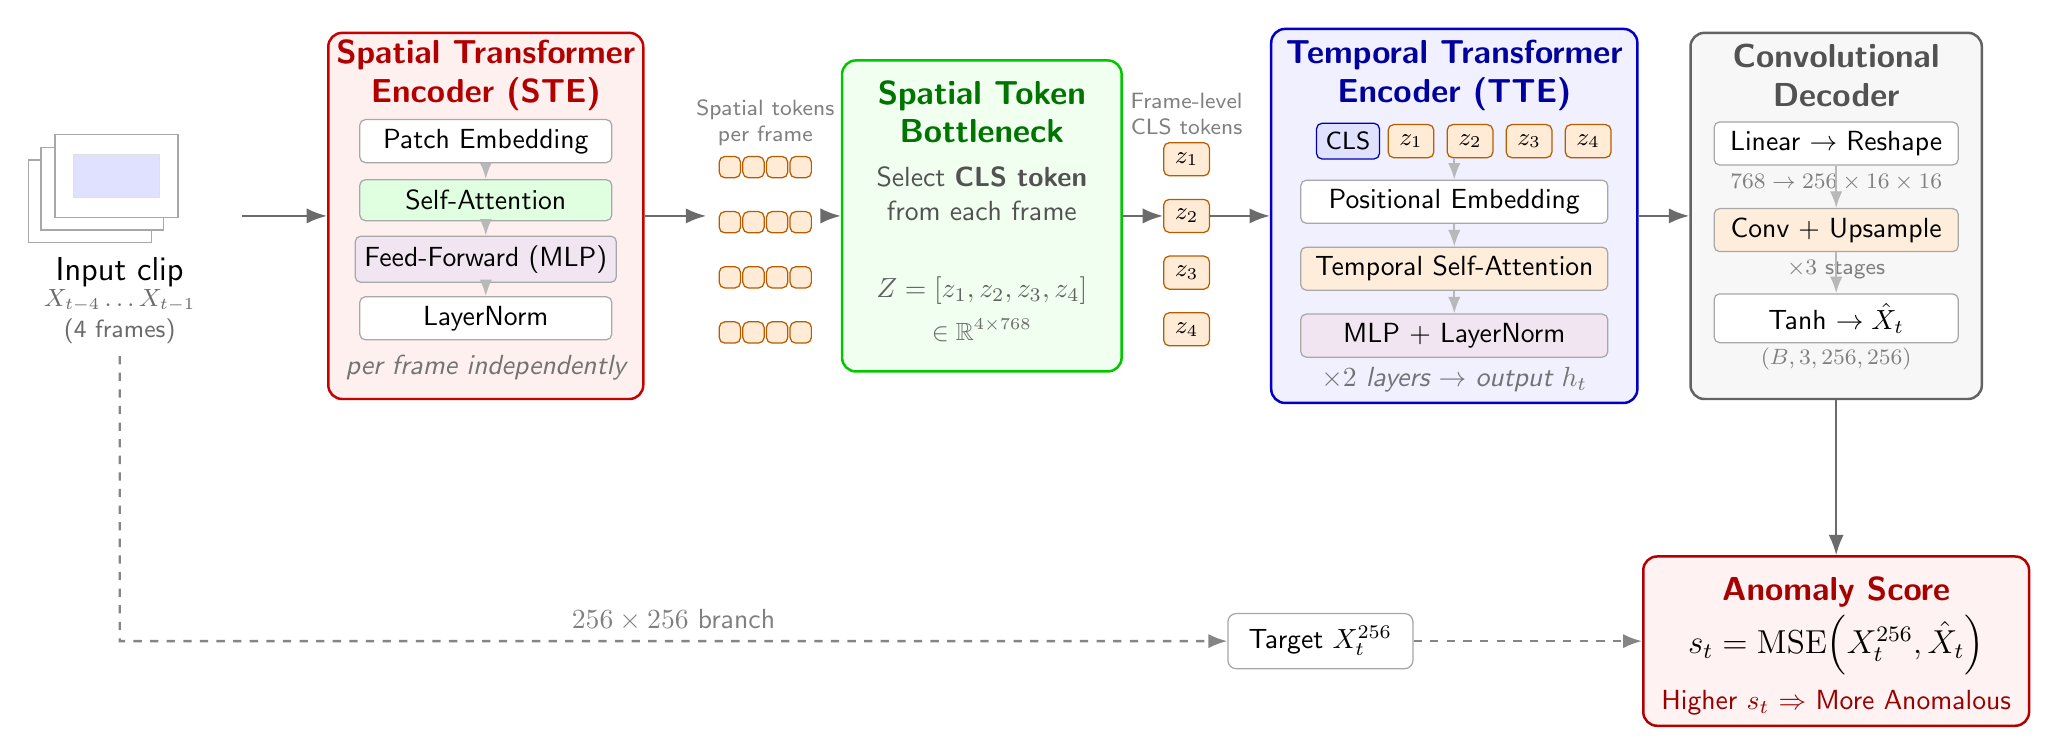
\begin{tikzpicture}[
    >=Latex,
    font=\sffamily,
    main/.style={-{Latex[length=2.6mm]}, line width=0.85pt, draw=black!58},
    innerarrow/.style={-{Latex[length=2.1mm]}, line width=0.72pt, draw=black!28},
    branch/.style={-{Latex[length=2.4mm]}, line width=0.82pt, draw=black!48, dashed},
    panel/.style={
        draw=#1!78!black,
        fill=#1!6,
        rounded corners=5pt,
        line width=0.9pt,
        minimum width=3.25cm,
        minimum height=4.15cm,
        align=center
    },
    title/.style={font=\sffamily\bfseries\large, align=center},
    block/.style={
        draw=black!34,
        fill=#1,
        rounded corners=2pt,
        minimum width=2.75cm,
        minimum height=0.52cm,
        font=\sffamily\normalsize,
        align=center,
        line width=0.45pt
    },
    token/.style={
        draw=orange!72!black,
        fill=orange!16,
        rounded corners=2pt,
        minimum width=0.58cm,
        minimum height=0.42cm,
        font=\sffamily\small,
        line width=0.45pt
    },
    clstok/.style={
        draw=blue!70!black,
        fill=blue!12,
        rounded corners=2pt,
        minimum width=0.64cm,
        minimum height=0.42cm,
        font=\sffamily\small,
        line width=0.45pt
    },
    note/.style={font=\sffamily\small, text=black!58, align=center},
    smallnote/.style={font=\sffamily\footnotesize, text=black!50, align=center}
]

% Coordinates
\coordinate (inputC) at (0, 3.15);
\coordinate (steC) at (4.65, 3.15);
\coordinate (tokC) at (8.20, 3.15);
\coordinate (botC) at (10.95, 3.15);
\coordinate (outTokC) at (13.55, 3.15);
\coordinate (tteC) at (16.95, 3.15);
\coordinate (decC) at (21.80, 3.15);
\coordinate (targetC) at (15.25, -2.25);
\coordinate (scoreC) at (21.80, -2.25);

% ---------------------------------------------------------------------
% Input clip
% ---------------------------------------------------------------------
\begin{scope}[shift={(inputC)}]
    \foreach \x/\y/\fc in {-0.34/0.18/blue!7, -0.18/0.34/blue!9, 0/0.50/blue!12} {
        \draw[draw=black!34, fill=white, line width=0.45pt]
            (\x-0.82,\y-0.52) rectangle ++(1.56,1.05);
        \draw[draw=black!12, fill=\fc, line width=0.35pt]
            (\x-0.58,\y-0.27) rectangle ++(1.08,0.55);
    }
    \node[font=\sffamily\large] at (0,-0.72) {Input clip};
    \node[note] at (0,-1.28) {$X_{t-4}\ldots X_{t-1}$\\(4 frames)};
\end{scope}

% ---------------------------------------------------------------------
% Spatial Transformer Encoder
% ---------------------------------------------------------------------
\node[panel=red, minimum width=4.00cm, minimum height=4.65cm] (ste) at (steC) {};
\node[title, text=red!70!black] at ($(steC)+(0,1.78)$)
    {Spatial Transformer\\Encoder (STE)};
\node[block=white, minimum width=3.20cm]     (ste1) at ($(steC)+(0,0.95)$) {Patch Embedding};
\node[block=green!12, minimum width=3.20cm]  (ste2) at ($(steC)+(0,0.20)$) {Self-Attention};
\node[block=violet!10, minimum width=3.20cm] (ste3) at ($(steC)+(0,-0.55)$) {Feed-Forward (MLP)};
\node[block=white, minimum width=3.20cm]     (ste4) at ($(steC)+(0,-1.30)$) {LayerNorm};
\node[font=\sffamily\itshape\normalsize, text=black!55] at ($(steC)+(0,-1.93)$)
    {per frame independently};

\draw[innerarrow] (ste1.south) -- (ste2.north);
\draw[innerarrow] (ste2.south) -- (ste3.north);
\draw[innerarrow] (ste3.south) -- (ste4.north);

% ---------------------------------------------------------------------
% Spatial tokens before bottleneck
% ---------------------------------------------------------------------
\node[smallnote] at ($(tokC)+(0,1.18)$) {Spatial tokens\\per frame};
\foreach \r/\y in {1/0.62,2/-0.08,3/-0.78,4/-1.48} {
    \foreach \x in {-0.45,-0.15,0.15,0.45} {
        \node[token, minimum width=0.27cm, minimum height=0.27cm, inner sep=0pt] at ($(tokC)+(\x,\y)$) {};
    }
}

% ---------------------------------------------------------------------
% Spatial Token Bottleneck
% ---------------------------------------------------------------------
\node[panel=green, minimum width=3.55cm, minimum height=3.95cm] (bot) at (botC) {};
\node[title, text=green!45!black] at ($(botC)+(0,1.32)$)
    {Spatial Token\\Bottleneck};
\node[font=\sffamily\normalsize, text=black!68, align=center] at ($(botC)+(0,0.28)$)
    {Select \textbf{CLS token}\\from each frame};
\node[font=\sffamily\normalsize, text=black!62] at ($(botC)+(0,-0.95)$)
    {$Z=[z_1,z_2,z_3,z_4]$};
\node[note] at ($(botC)+(0,-1.45)$) {$\in \mathbb{R}^{4 \times 768}$};

% ---------------------------------------------------------------------
% Frame-level CLS tokens after bottleneck
% ---------------------------------------------------------------------
\node[smallnote] at ($(outTokC)+(0,1.30)$) {Frame-level\\CLS tokens};
\node[token] (z1) at ($(outTokC)+(0,0.72)$) {$z_1$};
\node[token] (z2) at ($(outTokC)+(0,0.00)$) {$z_2$};
\node[token] (z3) at ($(outTokC)+(0,-0.72)$) {$z_3$};
\node[token] (z4) at ($(outTokC)+(0,-1.44)$) {$z_4$};

% ---------------------------------------------------------------------
% Temporal Transformer Encoder
% ---------------------------------------------------------------------
\node[panel=blue, minimum width=4.65cm, minimum height=4.75cm] (tte) at (tteC) {};
\node[title, text=blue!62!black] at ($(tteC)+(0,1.78)$)
    {Temporal Transformer\\Encoder (TTE)};

\node[clstok] at ($(tteC)+(-1.35,0.95)$) {CLS};
\foreach \i/\x in {1/-0.55,2/0.20,3/0.95,4/1.70} {
    \node[token] at ($(tteC)+(\x,0.95)$) {$z_\i$};
}
\node[block=white, minimum width=3.90cm]      (tte1) at ($(tteC)+(0,0.18)$) {Positional Embedding};
\node[block=orange!14, minimum width=3.90cm]  (tte2) at ($(tteC)+(0,-0.67)$) {Temporal Self-Attention};
\node[block=violet!10, minimum width=3.90cm]  (tte3) at ($(tteC)+(0,-1.52)$) {MLP + LayerNorm};
\node[font=\sffamily\itshape\normalsize, text=black!55] at ($(tteC)+(0,-2.08)$)
    {$\times 2$ layers $\rightarrow$ output $h_t$};

\draw[innerarrow] ($(tteC)+(0,0.74)$) -- (tte1.north);
\draw[innerarrow] (tte1.south) -- (tte2.north);
\draw[innerarrow] (tte2.south) -- (tte3.north);

% ---------------------------------------------------------------------
% Convolutional Decoder
% ---------------------------------------------------------------------
\node[panel=gray, minimum width=3.70cm, minimum height=4.65cm] (dec) at (decC) {};
\node[title, text=black!68] at ($(decC)+(0,1.78)$)
    {Convolutional\\Decoder};
\node[block=white, minimum width=3.10cm]      (dec1) at ($(decC)+(0,0.92)$) {Linear $\rightarrow$ Reshape};
\node[smallnote] at ($(decC)+(0,0.42)$) {$768 \rightarrow 256 \times 16 \times 16$};
\node[block=orange!14, minimum width=3.10cm]  (dec2) at ($(decC)+(0,-0.18)$) {Conv + Upsample};
\node[smallnote] at ($(decC)+(0,-0.68)$) {$\times 3$ stages};
\node[block=white, minimum width=3.10cm]      (dec3) at ($(decC)+(0,-1.30)$) {Tanh $\rightarrow \hat{X}_t$};
\node[smallnote] at ($(decC)+(0,-1.82)$) {$(B,3,256,256)$};

\draw[innerarrow] (dec1.south) -- (dec2.north);
\draw[innerarrow] (dec2.south) -- (dec3.north);

% ---------------------------------------------------------------------
% Target branch and anomaly score
% ---------------------------------------------------------------------
\node[draw=black!35, fill=white, rounded corners=3pt,
    minimum width=2.35cm, minimum height=0.70cm,
    font=\sffamily\normalsize, line width=0.45pt] (target) at (targetC)
    {Target $X_t^{256}$};

\node[draw=red!70!black, fill=red!5, rounded corners=5pt,
    minimum width=4.90cm, minimum height=2.15cm,
    line width=0.9pt]
    (score) at (scoreC) {};
\node[title, text=red!65!black] at ($(scoreC)+(0,0.62)$) {Anomaly Score};
\node[font=\sffamily\large] at ($(scoreC)+(0,-0.05)$)
    {$s_t=\mathrm{MSE}\!\left(X_t^{256},\hat{X}_t\right)$};
\node[font=\sffamily\normalsize, text=red!60!black] at ($(scoreC)+(0,-0.78)$)
    {Higher $s_t$ $\Rightarrow$ More Anomalous};

% ---------------------------------------------------------------------
% Main flow
% ---------------------------------------------------------------------
\draw[main] ($(inputC)+(1.55,0)$) -- (ste.west);
\draw[main] (ste.east) -- ($(tokC)+(-0.75,0)$);
\draw[main] ($(tokC)+(0.75,0)$) -- (bot.west);
\draw[main] (bot.east) -- (z2.west);
\draw[main] (z2.east) -- (tte.west);
\draw[main] (tte.east) -- (dec.west);
\draw[main] (dec.south) -- (score.north);

% Target branch
\draw[branch] ($(inputC)+(0,-1.78)$) -- ($(inputC)+(0,-5.40)$)
    -- node[above, midway, font=\sffamily\normalsize, text=black!50]
        {$256 \times 256$ branch}
    (target.west);
\draw[branch] (target.east) -- (score.west);

\end{tikzpicture}
\end{document}
